\documentclass[conference]{IEEEtran}
\IEEEoverridecommandlockouts{}
% The preceding line is only needed to identify funding in the first footnote. If that is unneeded, please comment it out.
\usepackage{cite}
\renewcommand{\citepunct}{,\penalty\citepunctpenalty\,}
\usepackage{amsmath,amssymb,amsfonts}
\usepackage{algorithmic}
\usepackage{graphicx}
\usepackage{textcomp}
\usepackage{xcolor}
\usepackage{footnote}
\usepackage{url}
\usepackage{hyperref}
\usepackage{subcaption}               % subfiguren
\def\BibTeX{{\rm B\kern-.05em{\sc i\kern-.025em b}\kern-.08em
\kern-.1667em\lower.7ex\hbox{E}\kern-.125emX}}

\usepackage{scrextend}

% \setlength{\parskip}{8pt}
\begin{document}

\title{\textbf{\LARGE Time Is Running Out\\
        \large Assessing Temporal Privacy of Privacy Zones in Fitness Tracking Social Networks}
}

\author{
    \IEEEauthorblockN{Deleu, Wout}
    \IEEEauthorblockA{
        \textit{KU Leuven, Campus Rabot} \\
        Ghent, Belgium
    }
}
\maketitle

\begin{abstract}
    In a society where social media is so ubiquitous, the privacy concerns
    around them are more relevant than ever.  During this article, the main
    focus will be on the privacy policies of fitness trackers. Fitness trackers are
    platforms which store and display data related to sport activities. These can
    be shared with other users. This data may include heart rate, GPS-locations,
    etc. This type of data sharing can however cause unintentionally sharing of
    sensitive information, like home addresses.

    Most fitness tracking networks are aware of this danger and implement a series
    of countermeasures to prevent this. One of these countermeasures is the use of
    Endpoint Privacy Zones (EPZs) which is a zone around a sensitive location,
    which hides the part of the trajectory which ends or begins in this zone.
    Previous research has shown that it is possible to retrieve the sensitive
    location using the available data from the activity. Dhondt et al.\ showed that
    based on the total distance travelled, the sensitive location can be retrieved
    using an `inference attack'~\cite{Dhondt}. This study will investigate the
    possibilities of such inference attacks using other data than the distance. We
    want to recreate the results as good as possible using the speed and tempo of
    the activity, together with GPS-locations. This can result in an attack model
    with a success rate up to 75\%. This is lower than the previous implementation
    of Dhondt et al., but this shows that the attack is still possible under
    circumstances where the distance is rendered unusable. This also includes some
    countermeasure described by Dhondt et al. But countermeasures like enlarging
    the EPZ or shifting endpoints still have effect.\vspace{6pt}

\end{abstract}
\begin{IEEEkeywords}
    fitness-trackers, privacy, GPS-locations, endpoint privacy zone, inference attack
\end{IEEEkeywords}

\section{\textbf{Introduction}}
Social media has become virtually indispensable in today's modern life and
branches out into a lot of facets, including social networking, media sharing
networks, etc, but also the branch of fitness trackers. This rise of these new
media, however, also brings unintended but significant privacy concerns.

The focus of this thesis is on privacy within these fitness trackers, more
specific platforms that use GPS locations, such as
Strava\footnote{\label{fn:strava}\url{https://www.strava.com/}}, Nike Run Club,
etc. These are platforms where individuals can share sports activities such as
running, cycling, hiking, \ldots with each other. The general concept is here
that when you perform a sports activity, you make it available to your
followers and friends. The sports activities will naturally release certain
data to those other users, which could possibly have negative effects on the
users privacy. For example leaking the home address of the user, which can lead
to stalking and burglary~\cite{Sportapp72:online, Cyclistw89:online}. There are
even some reports about military bases being discovered using the Strava
heatmap~\cite{Fitnesst33:online}.
\begin{figure}[h]
    \centering
    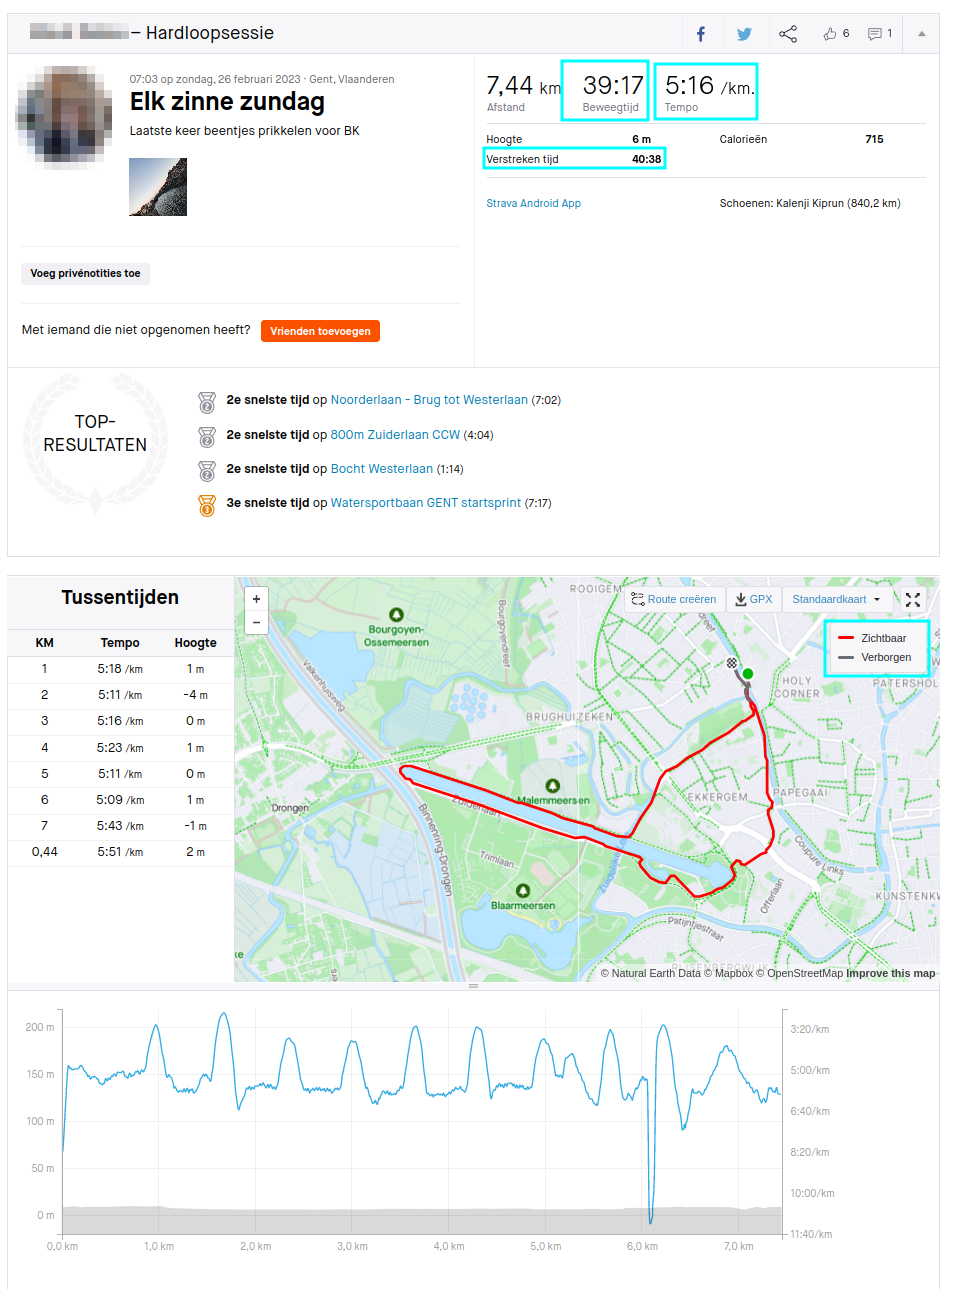
\includegraphics[width=\linewidth]{fig/VoorbeeldActiviteiten/VoorbeeldActiviteit_Personal.png}
    \caption{Example of a Strava activity}\label{fig:activity}
\end{figure}

Fitness trackers each implement ways to improve user privacy. Perhaps the most
easy way to think of is perhaps the ability to hide activities from a selection
of people (e.g., anyone who is not a follower). Thus, only the people whom the
user explicitly allows to view activities. A more complex alternative is to use
EPZs. Hereby will a portion of the displayed route be hidden for external
viewers. Part of the route is cut off, so to speak. The real starting and
ending points will lie inside the truncated part. New points will be generated,
on the edge of the circle, which for the external observer will represent the
beginning and end. The beginning and end part of the route will thus become
invisible to the other users. Due to the presence of all these attempts at
privacy enhancements, it is noticeable that the developers of the platforms are
very aware of the potential dangers. However, there is a trade-off to be made
when implementing between the usability of the platform, and the privacy of the
end user. The more data is released, the greater the chance of potentially
sensitive info being passed along. On the other hand, when omitting
information, the usability and presence of useful data of the platform is
greatly diminished.

In this study, we consider whether there is a possibility to retrieve hidden
locations of an activity, despite the use of an EPZ as privacy security
mechanism. Some ways to bypass the EPZ using other metadata such as elevation
data and distances have been described in the past~\cite{Verdonck_2022, Dhondt,
    sec18has3:online}. This thesis goes into more detail on the use of velocity
data. As a base for this attack, we use the inference attack, which was
described by Dhondt et al. We investigate whether this attack is still possible
when omitting certain data, and thus by the use of alternative data. The focus
of this study is mainly on velocity-based data.

To achieve this objective, we must first examine the attack model according to
Dhondt el al. Then we can describe different possible alternative attack
scenarios, and for each work out the calculations necessary in order for this
scenario to be possible. Before we can test and analyze the attack, we must
consider the possible errors in the used dataset. We also perform an analysis
on the difference between the calculated distances, and the values derived
according to the calculations of Dhondt et al. So can we estimate the
effectiveness of the attack a priori to some extent. Only then do we execute
the attack, evaluate the attacks and form meaningful conclusions.

\section{\textbf{Background}}
The data used to test the effectiveness the attack and perform experiments
comes from the popular fitness tracker Strava\footref{fn:strava}. This is a
social network where all types of athletes can share their activities. This
includes running, walking, cycling, swimming, \ldots The collected data is
filtered according to the perspective of a possible attacker. Not all data
turns out to be useful. Only data that could reveal sensitive information
regarding residence is retained. This will therefore mean that only activities
that contain relevant GPS information will be considered, so only
\textit{runs}, \textit{hikes}, \textit{walks}, and \textit{bike rides}.
\begin{figure}[h]
    \centering
    
\includegraphics[width=0.6\linewidth]{fig/Logo_Strava.png}
    \caption{Strava logo~\cite{strava_companie}}\label{fig:stravalogo}
\end{figure}

Some visbible data on an activity, which can also be found on
Figure~\ref{fig:activity}, are the distance, the duration, the average speed,
etc. The average speed forms the core to the attack which we will describe in
this article. This will be calculated as the total distance divided by the
moving time of the athlete. Fitness trackers receive raw data from the devices.
This data must therefore be processed before it is usefull fo the users.
Especially GPS-data, which is can be exposed to a lot of faults and noise.
There are three types of GPS-faults, namely \textit{GPS drift}, \textit{GPS
    signal loss} and \textit{GPS bounce}. GPS-drift is a phenomenon where a user's
GPS location deviates from the effective location. This may be caused by
densely built environments, and natural factors such as tall trees. GPS
bouncing is a phenomenon caused mainly by tall buildings. In this situation,
the GPS signal will bounce in between buildings on its way to the device from
the satellite. The extra delay that the bounces bring along causes the device
to mistakenly think it has traveled some additional distance. The outcome of
the trajectory is then unpredictable, leading to a `cluster' of GPS points. A
last phenomenon that can occur is GPS signal loss. This occurs when the user's
signal is lost, and a new signal is only received at a later time stamp,
causing a jump. A second cause that can lead to signal loss, which especially
applies to fitness trackers, is the ability to pause an activity. I When the
activity is resumed again, there will be a jump in GPS locations, which may
lead to miscalculation of distance.

\begin{figure}[h]
    \centering
    \begin{subfigure}[b]{.48\linewidth}
        \centering
        \caption{GPS bounce example}
        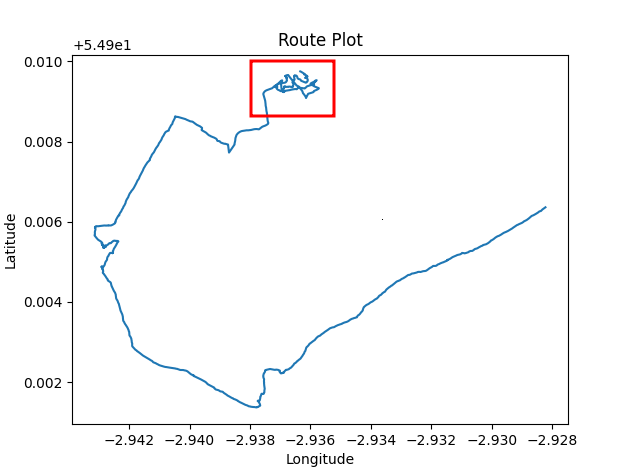
\includegraphics[width=\textwidth]{fig/Afwijkingen&Analyses/Crooked Routes/Crooked GPS Route_Cart.png}
    \end{subfigure}
    \begin{subfigure}[b]{.38\linewidth}
        \centering
        \caption{GPS signal loss}
        \includegraphics[width=1\textwidth]{fig/Afwijkingen&Analyses/Crooked Routes/1_Full_withArrow.png}
    \end{subfigure}
    \begin{subfigure}[b]{0.6\linewidth}
        \centering
        \caption{GPS drift}
        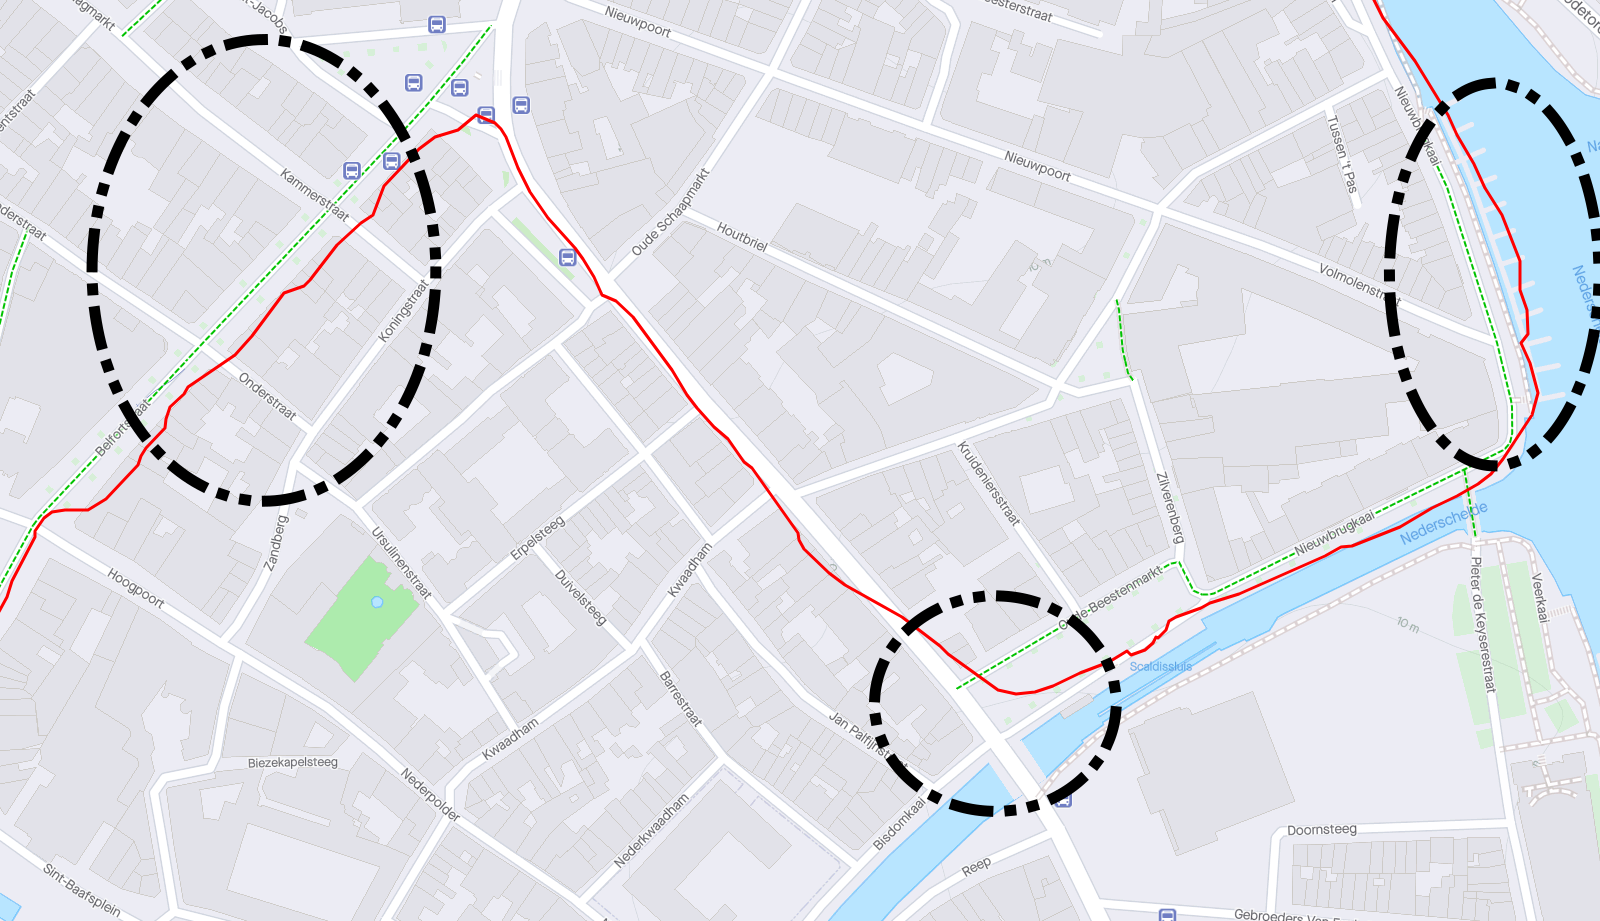
\includegraphics[width=\textwidth]{fig/Afwijkingen&Analyses/Crooked Routes/GPS-Drift.png}
    \end{subfigure}
    \caption{Possible GPS-faults}
\end{figure}

Some techniques can be used to improve the overall accuracy of the GPS data,
and so improve the effectiveness of the attack. The main technique used in this
thesis is \textit{smoothing}, and the hypothesis is that fitnessplatformen use
this technique as well. This is a technique to enhance the accuracy and
reliability of GPS data. There are different implementations of GPS smoothing,
but the one used in this context is moving average filtering. This method
calculates an average position by considering a sliding window of the most
recent GPS measurements. By averaging multiple measurements over a certain time
period, the effects of noise and temporary inaccuracies can be mitigated,
resulting in a smoother and more reliable trajectory. The size of the window
can be chosen. The larger the window, the less accurate the trajectory will be,
but the more noise will be countered. This technique is especially useful to
counter GPS bouncing and GPS drift.

AANVULLEN EPZ + PREVIOUS WORK
\section{\textbf{Setting of the attack}}\

\section{\textbf{Used Data}}

\section{\textbf{Results and Conclusions}}

\bibliographystyle{IEEEtran}
\bibliography{bibliografie_eng}
\end{document}